\documentclass[12pt,oneside,a4paper,english]{article}
\usepackage[T1]{fontenc}
\usepackage[utf8]{inputenc}
\usepackage[margin=2.25cm,headheight=26pt,includeheadfoot]{geometry}
\usepackage[danish]{babel}
\usepackage{listings}
\usepackage{color}
\usepackage{titlesec}
\usepackage{titling}
\usepackage[framed, numbered]{matlab-prettifier}
\usepackage{changepage}
\usepackage{amsmath}
\usepackage{hyperref}
\usepackage{enumitem}
\usepackage{graphicx}
\usepackage{fancyhdr}
\usepackage{lastpage}
\usepackage{caption}
\usepackage{tocloft}
\usepackage{setspace}
\usepackage{multirow}
\usepackage{titling}
\usepackage{float}
\usepackage{comment}
\usepackage{booktabs}
\usepackage{indentfirst}
\usepackage{lscape}
\usepackage{booktabs,caption}
\usepackage[flushleft]{threeparttable}
\usepackage[english]{nomencl}
\usepackage{xcolor}
\usepackage{lipsum}
\usepackage[backend=bibtex]{biblatex}
\addbibresource{document.bib}

% --- set footer and header ---
\pagestyle{fancy}
\fancyhf{}

\setlength{\parindent}{2em}
\title{CDIO1} % to reference as \title, dont use \maketitle
\makeatletter\let\Title\@title\makeatother



\lstset{language=Matlab,
style=Matlab-editor,
basicstyle=\normalsize\mlttfamily,
numbers=left,
numberstyle={\scriptsize\color{black}},			% size of the numbers
numbersep=0.5cm											
}

\newlist{steps}{enumerate}{1}
\setlist[steps, 1]{leftmargin=1.5cm,label = Step \arabic*:}
\renewcommand{\headrulewidth}{1pt}
\renewcommand{\footrulewidth}{1pt}

%\lhead{\Title}
\rhead{\nouppercase{\rightmark}}
\lhead{\Title}
\rfoot{
\includegraphics[height=1.25cm]{root/logo.pdf}} % right header logo
\setlength\headheight{16pt}
\setlength{\footskip}{50pt}
\lhead{\Title} %rightH title
\cfoot{\thepage}

% --- End of page settings ---



\begin{document}
\pagenumbering{roman} 

\begin{titlepage}
\begin{center}
\vspace{2cm}
%\textsc{ Danmarks Tekniske Universitet}\\[1.5cm]

\includegraphics[width=0.4\textwidth]{root/dtu.png}~\\[1cm]
\vspace{2cm}

\vspace{1.5cm}

% Title
\hrule
\vspace{.5cm}
{ \huge \bfseries CDIO3} % title of the report
\vspace{.5cm}

\hrule
\vspace{1.5cm}

\textsc{\textbf{Gruppe 25}}\\
\vspace{.5cm}
\centering

% add your name here
\begin{tabular}{|c|c|c|}
\hline
&&
\\

\includegraphics[scale=0.8]{figures/adam.png}
&

\includegraphics[scale=0.8]{figures/andreas.png}
&

\includegraphics[scale=0.8]{figures/bastian.png}
\\
Adam Harald Jørgensen
&
Andreas Engberg Carlsen
&
Bastian Emil Falk Larsen
\\
s200718
&
s205437
&
s195112\\
\hline
&&
\\

\includegraphics[scale=0.8]{figures/jens.png}
&

\includegraphics[scale=0.8]{figures/martin.png}
&

\includegraphics[scale=0.8]{figures/michael.png}
\\
Jens Skriver Kloster
&
Martin Lüthje Hermann
&
Michael Rene Lund Jensen
\\
s190265
&
s195127
&
s205460\\
\hline
\end{tabular}
\centering \today % Dags dato
\end{center}
\end{titlepage}

\newpage
\doublespacing
%\addcontentsline{toc}{section}{Table of Contents}
\renewcommand{\baselinestretch}{1}\normalsize
\tableofcontents
\renewcommand{\baselinestretch}{1}\normalsize
%\singlespacing
\thispagestyle{fancy} % force page style

\newpage
\pagenumbering{arabic} 
\fancyfoot[C]{Page \thepage\ of \pageref{EndOfText}}


\section{Resumé} \label{resume}
\input{sources/0_2_resume.tex}
\section{Indledning} \label{introduction}
IOOuteractive har stillet os en opgave, som går ud på at skulle lave et Monopoly Junior spil. Vi skal selv vurdere hvad der er vigtigst for at spille skal kunne køre, hvilket også betyder at regler må udelades.  
\newpage
\section{Krav} \label{demands}
\begin{figure}[h!]
\includegraphics[scale=1]{artifacts/Krav1.png}
\end{figure}
\begin{figure}[h!]
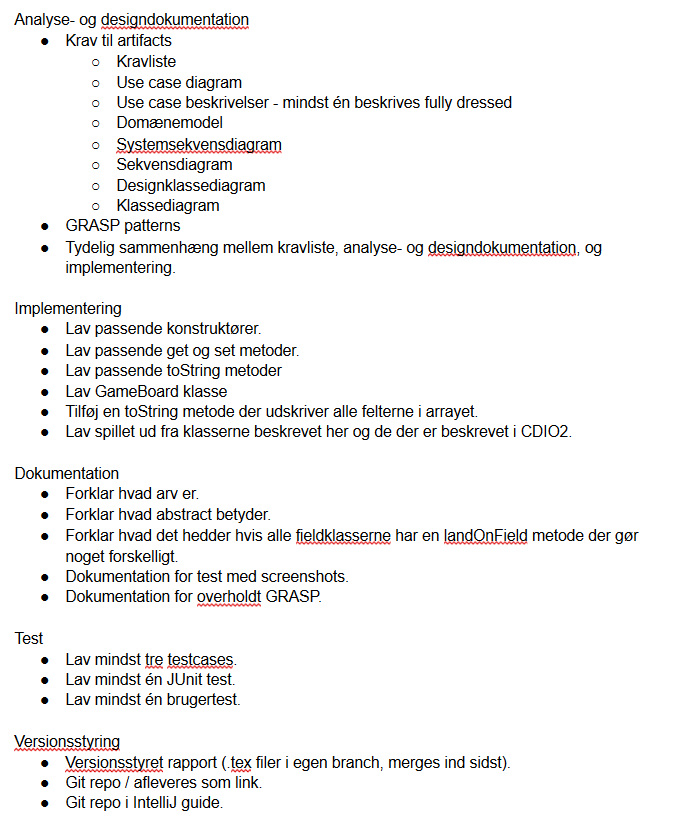
\includegraphics[scale=1]{artifacts/Krav2.png}
\end{figure}
\newpage
\section{Analyse} \label{analysis}
\subsection{Use case beskrivelser}
\begin{itemize}
	\item Spil spillet.
	
Spilleren spiller spillet.
\end{itemize}
Sub use case beskrivelser:
\begin{itemize}
	\item Indtast navn.\\ Spilleren indtaster sit navn.
	\item Vælg farve. \\ Spilleren vælger imellem et udvalg af farve.
	\item Rul terning. \\ Spilleren ruller med terningerne.
\end{itemize}

\subsection{Fully dressed Use case}
\begin{figure}[h!]
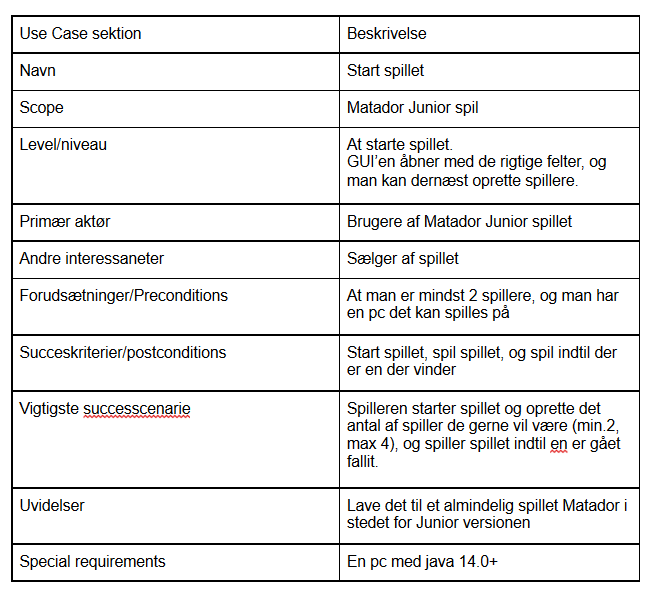
\includegraphics[scale=1]{artifacts/fullyDressed.png}
\end{figure}
\newpage
\subsection{Systemsekvensdiagram}
\begin{figure}
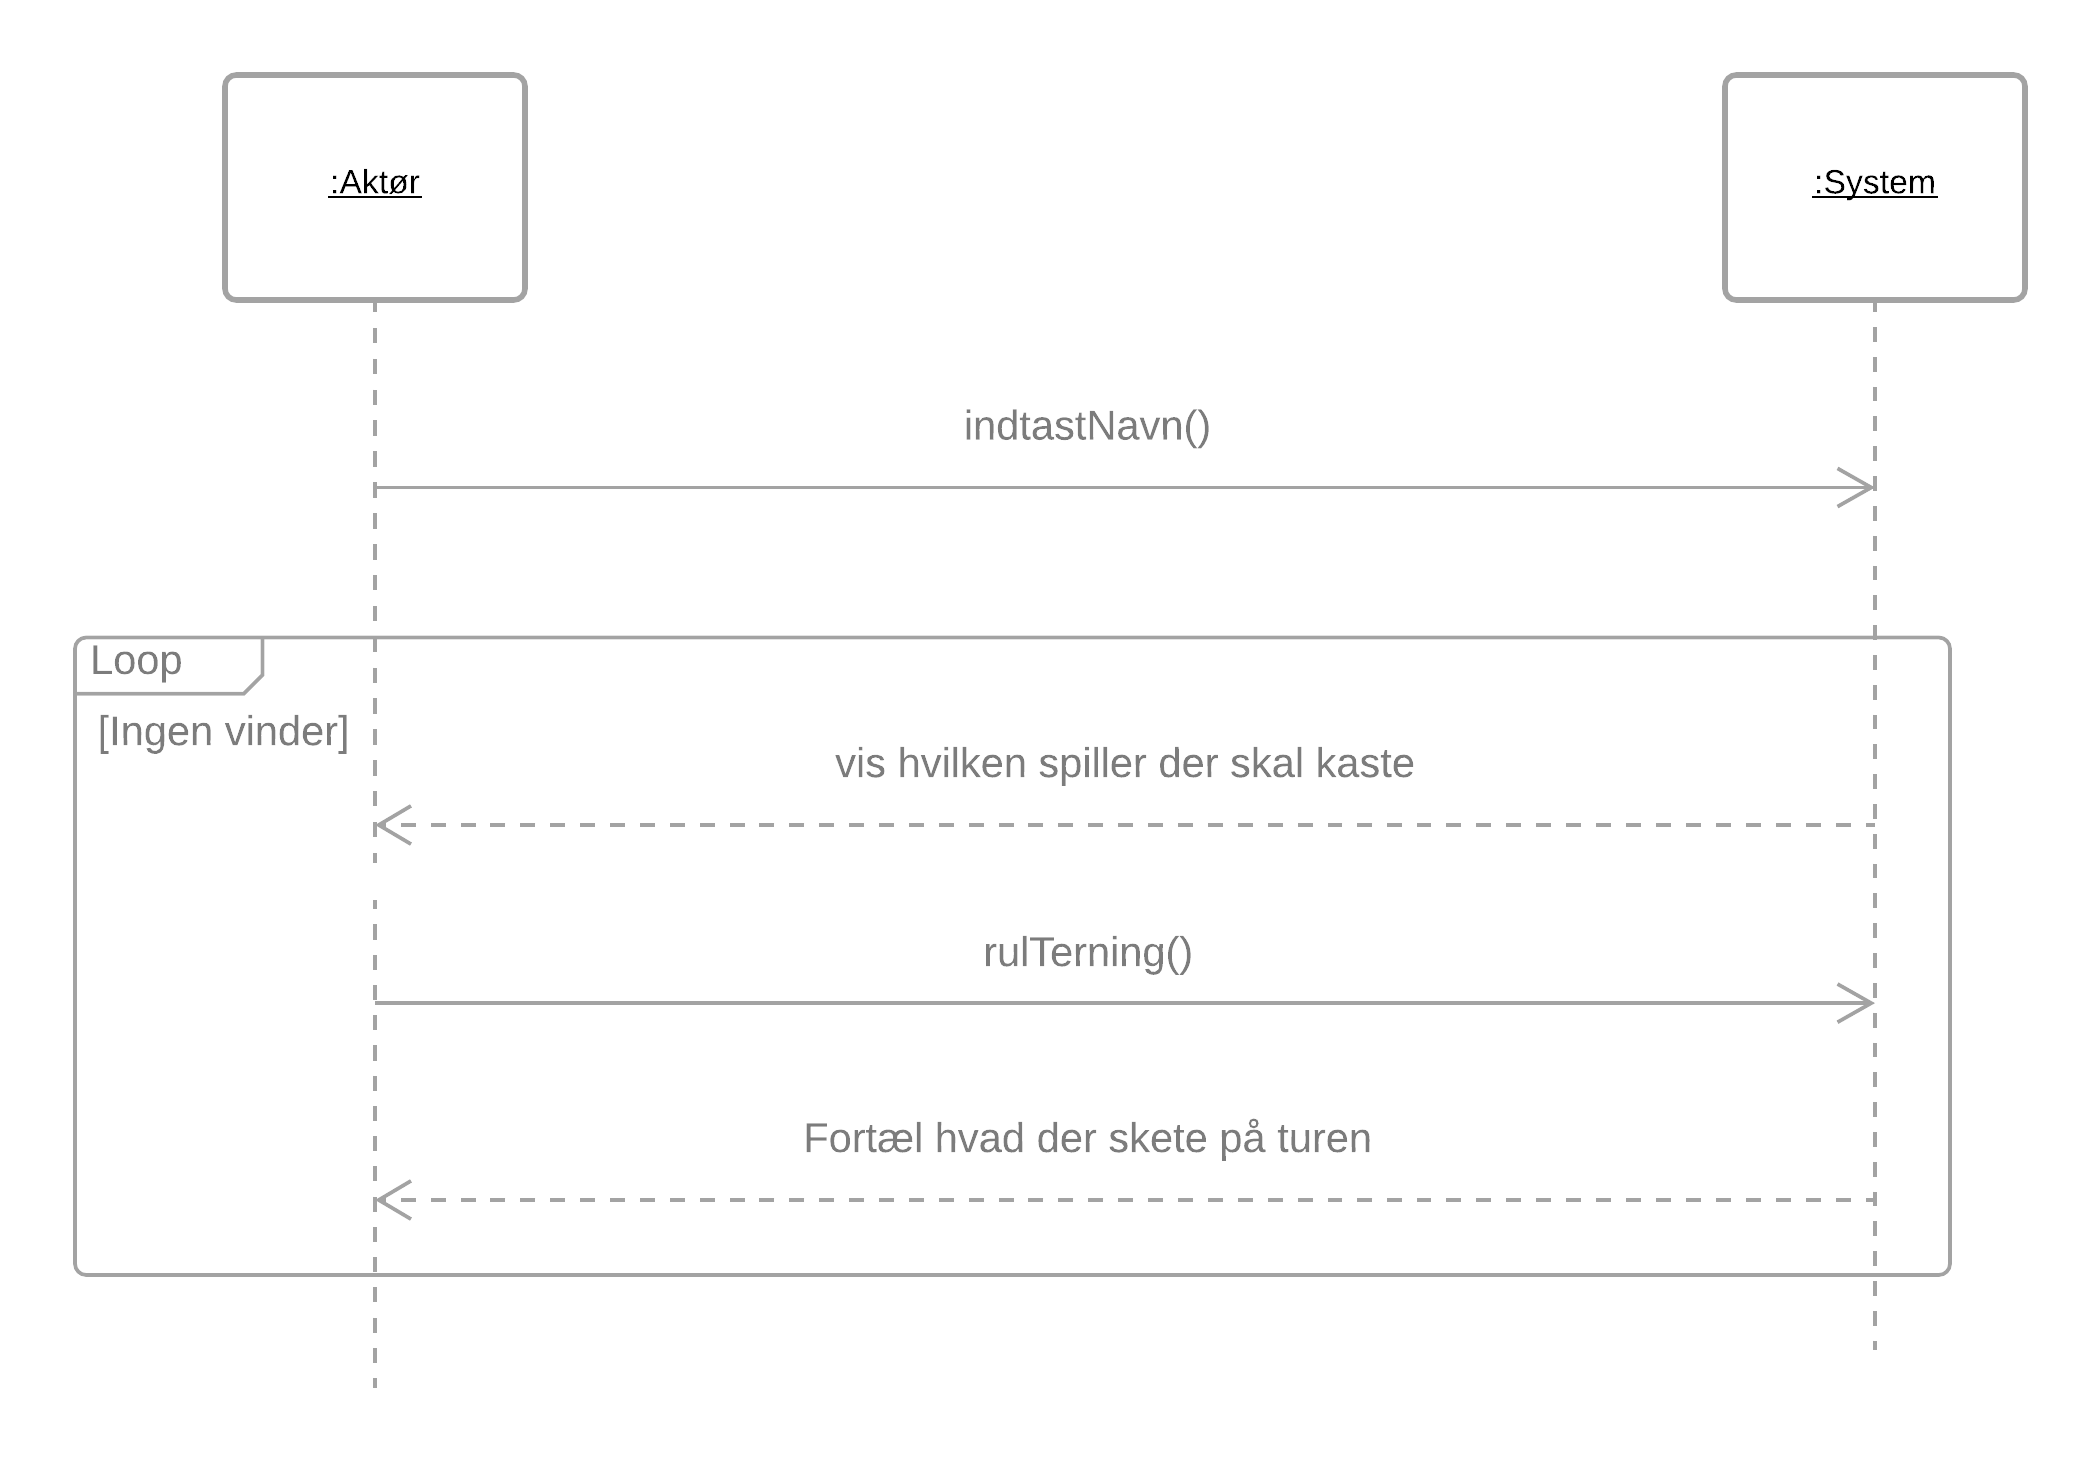
\includegraphics[scale=0.2]{artifacts/SSD.png}
\end{figure}
\newpage
\subsection{Designklassediagram}
\begin{figure}[h!]
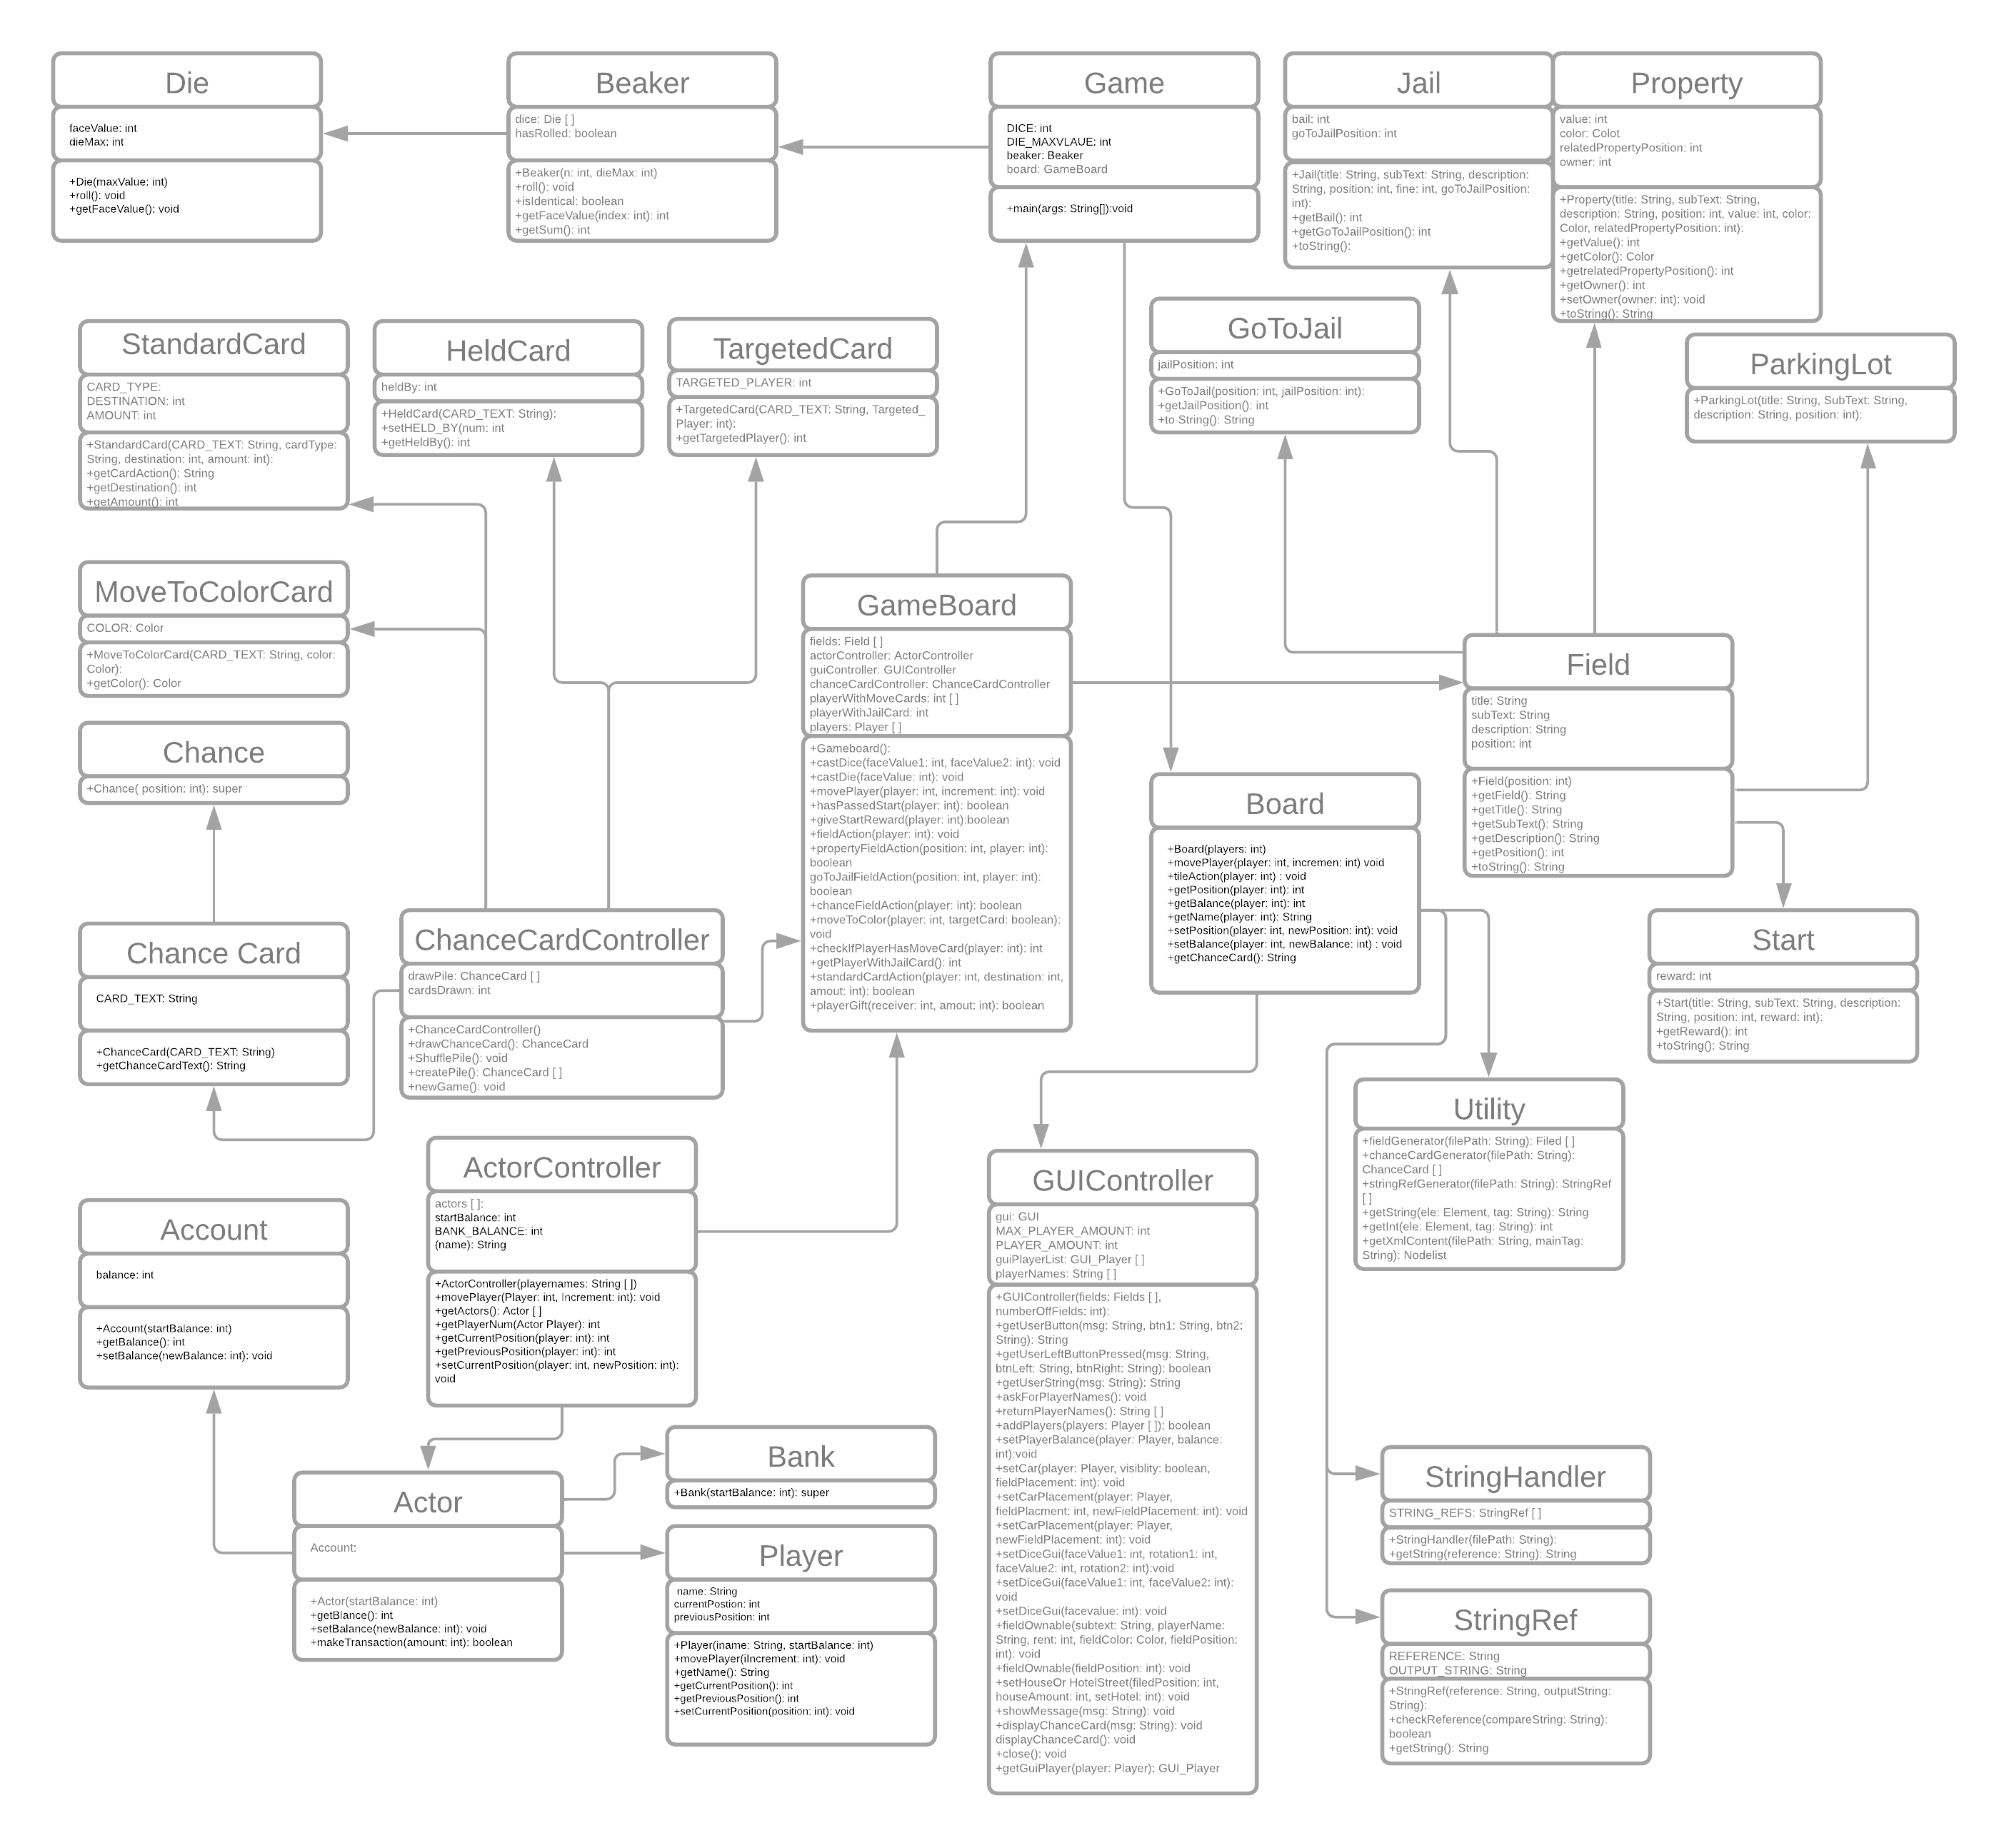
\includegraphics[scale=0.16]{artifacts/DCD.png}
\end{figure}
\newpage
\section{Design} \label{design}
\subsection{Klassediagram}
Klassediagrammet giver overblik over vores klasser i projektet. Vi har indset, at vi skal bruge mange objekter, der er variationer af samme type - f.eks. felter på spillepladen. Derfor gør vi brug af nedarvning. I tilfældet med felter er nedarvning smart, da nogle felter kan ejes af en spiller, mens andre ikke kan. Nogle felter har ingen konsekvenser (Parkeringsplads, fængsel), mens andre har (chance, start, ryk i fængsel, ejendomme).
Vi har valgt at bruge ordet \texttt{Actor} som generalisering. Dette skal ikke misforstås som aktør i kontekst af UML. I Monopoly Junior har banken egenskaber der til forveksling ligner en spillers, derfor har vi valgt at bruge nedarvning til dette, da vi bruger de samme methods til banken såvel som spilleren.
Utility er blevet flyttet udenfor diagrammet, da den ikke passer godt ind ellers. Utility bør muligvis omdøbes til Reader eller lignende, da det er mere beskrivende for hvad den gør - nemlig læser tekst- og XML-filer for at hente data til brug i andre dele af programmet. GameBoard og ChanceCardController skal begge bruge Utility for at generere adskillige objekter fra XML filer. GUIController har behov for at læse fra forskellige tekstfiler, og det bruger vi også Utility til.
\begin{figure}[h!]
\centering
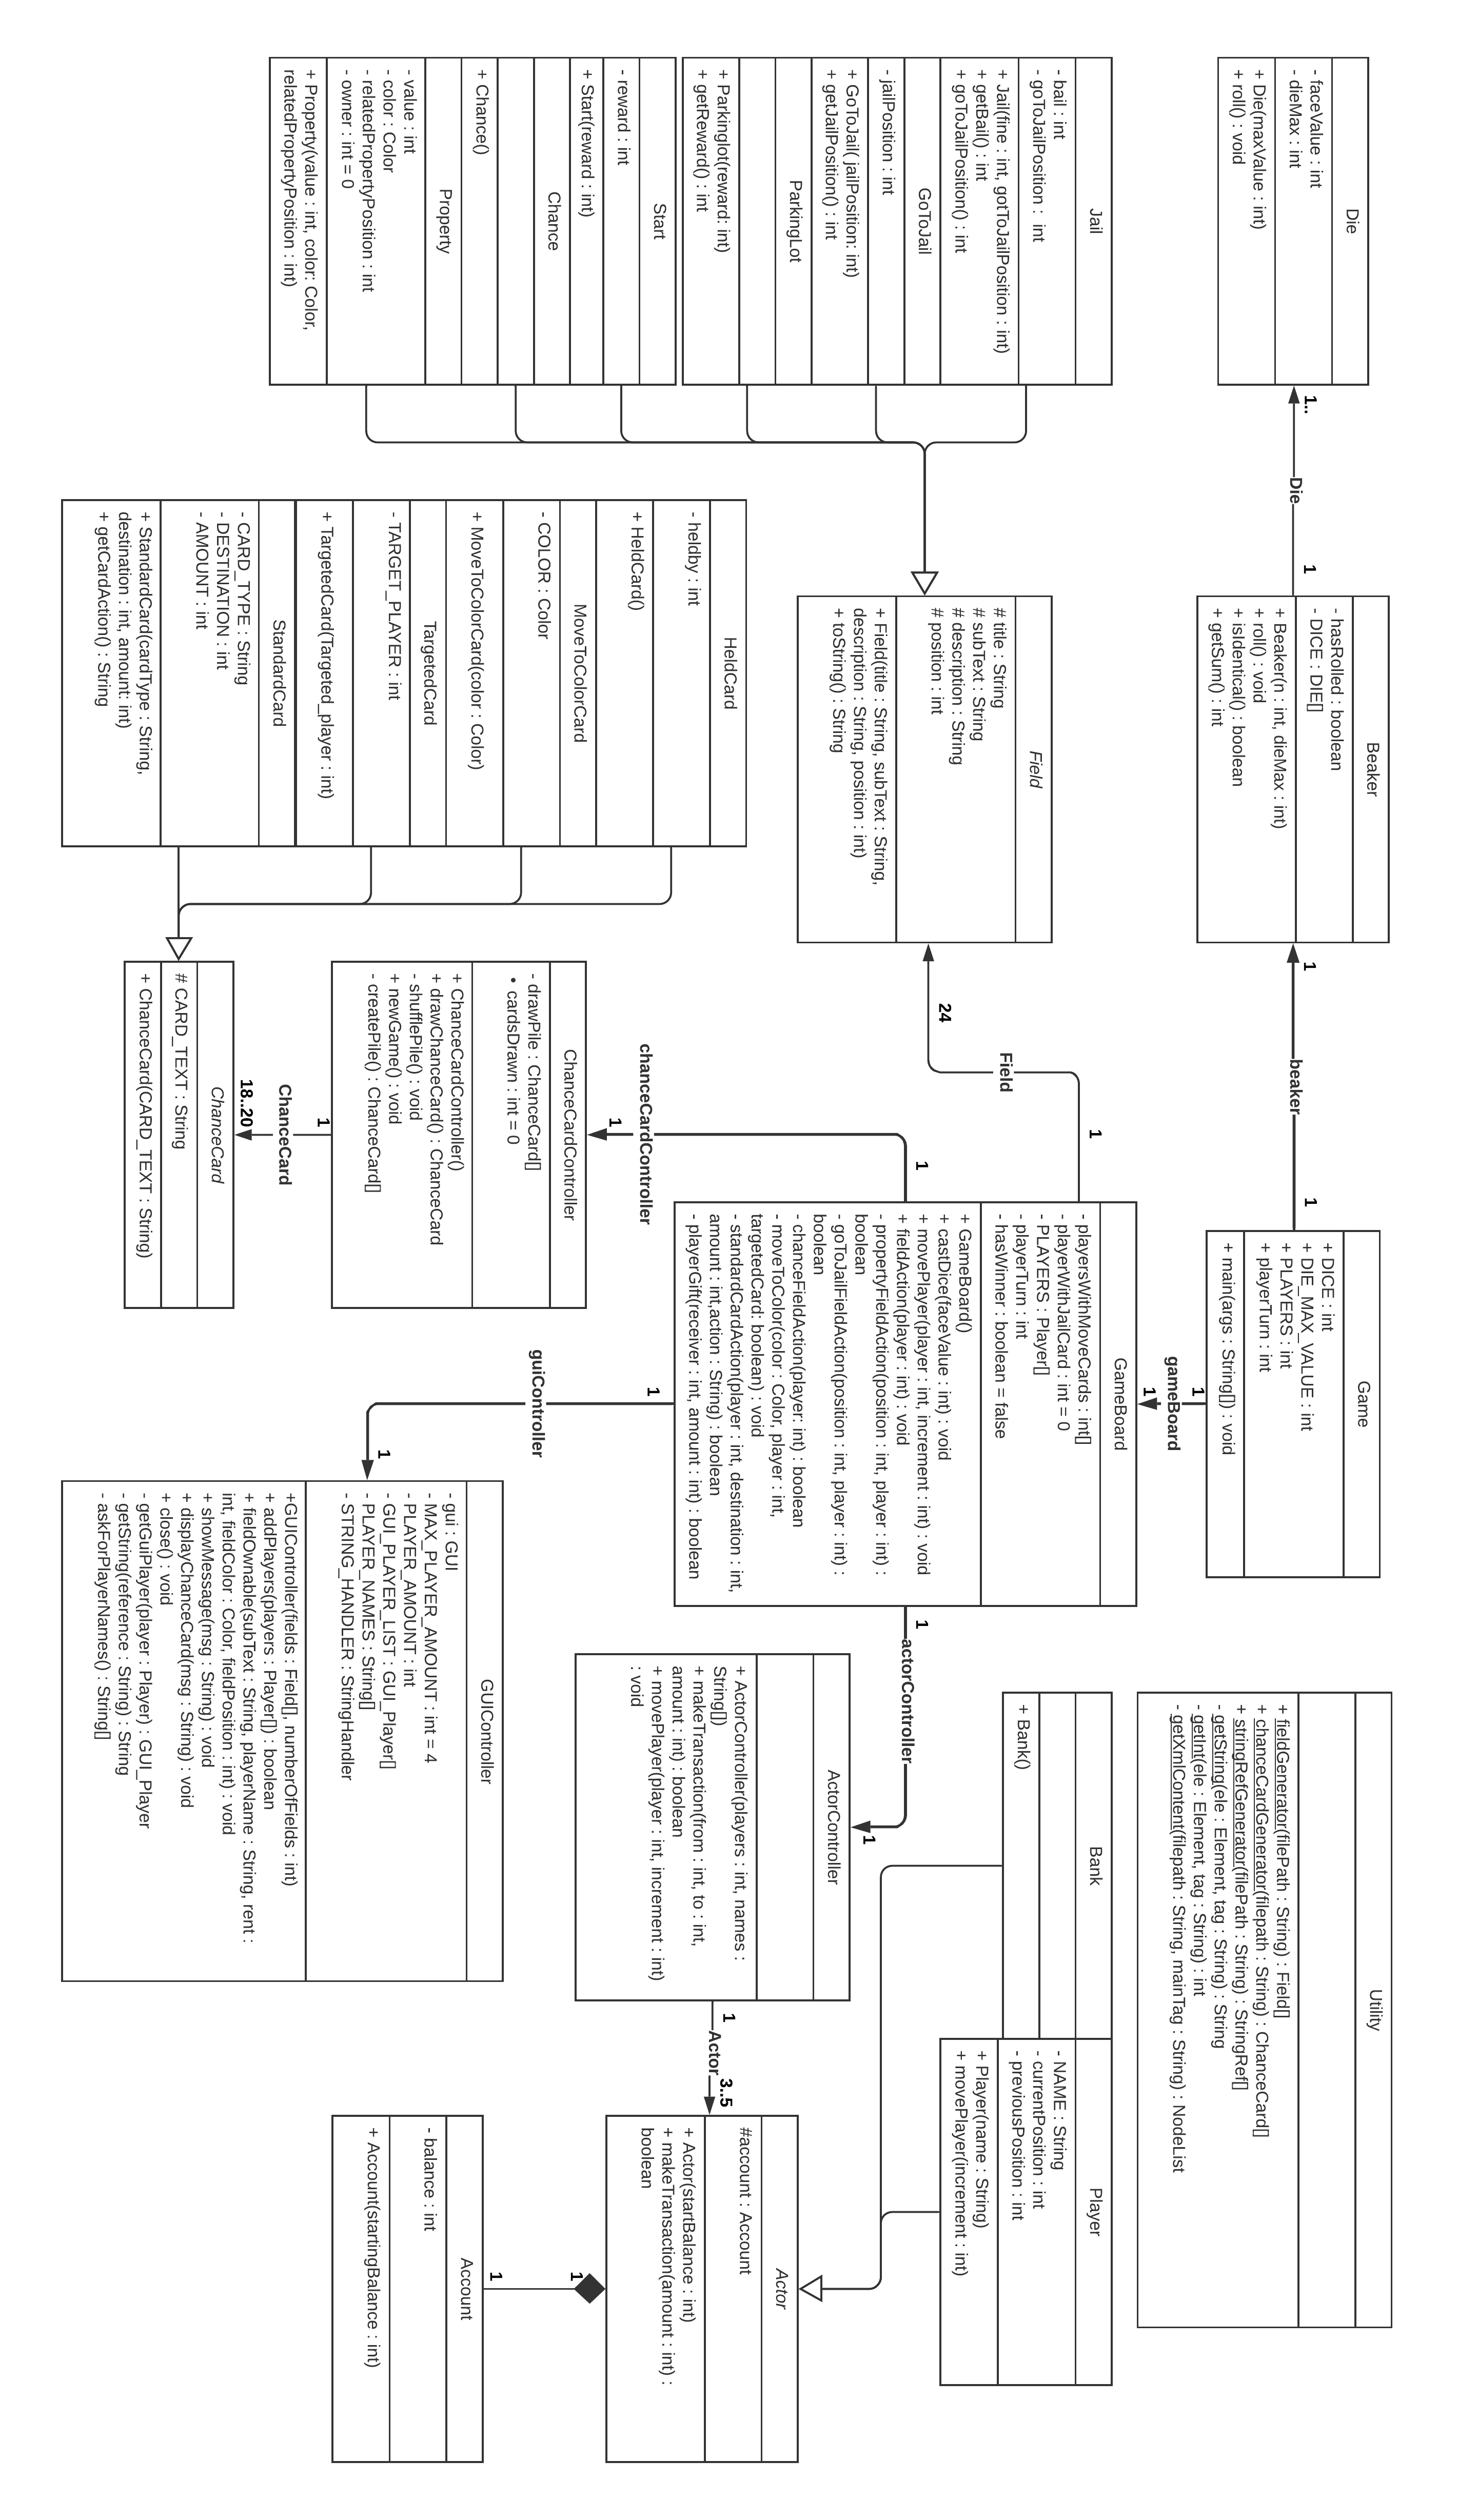
\includegraphics[scale=0.16]{artifacts/CD.png}
\end{figure}

\subsection{GUIController}
Klassen \texttt{GUIController} er den klasse som sørger for alt kommunikation til GUI’en, så vi kan nemmere hold styr på det hele ift. GRASP.
Dvs. der er kun 1 fil, man skal kigge i, når man vil kommunikere med GUI’en.
Klasse skal derud over være henholdsvis minimalistisk i den forstand af, at der skal helst ikke være mere end en 5-10 linjer kode i hver metode (nogle metoder undtaget), da det mest bare er kald, som går videre i systemet.


\subsection{ChanceCardController}
\texttt{ChanceCardController} bliver brugt til at holde styr på alle chancekort(dvs. holde en bunke kort, give mulighed for at trække et kort og blande bunken). Vi har valgt at lave en controller til dette, da det giver bedre mulighed for at overholde GRASP principperne. 
\subsection{GameBoard}
Denne klasse har vi bestemt til at være den centrale klasse der udfører det meste af handlingerne nødvendige for en spillerunde. \texttt{GameBoard} indeholder derfor både en \texttt{ActorController} til spillere og banken, en \texttt{GUIController} til at styre bruger interfacet samt et \texttt{Field} array. \texttt{GameBoard} fungerer som controller til felter, og indeholder derfor koden eksekveres for hver af felttyperne. 

Main bruger derfor kun en \texttt{Beaker} og en \texttt{GameBoard} klasse. 
\newpage
\subsection{Sekvensdiagram}
\begin{figure}[h!]
\centering
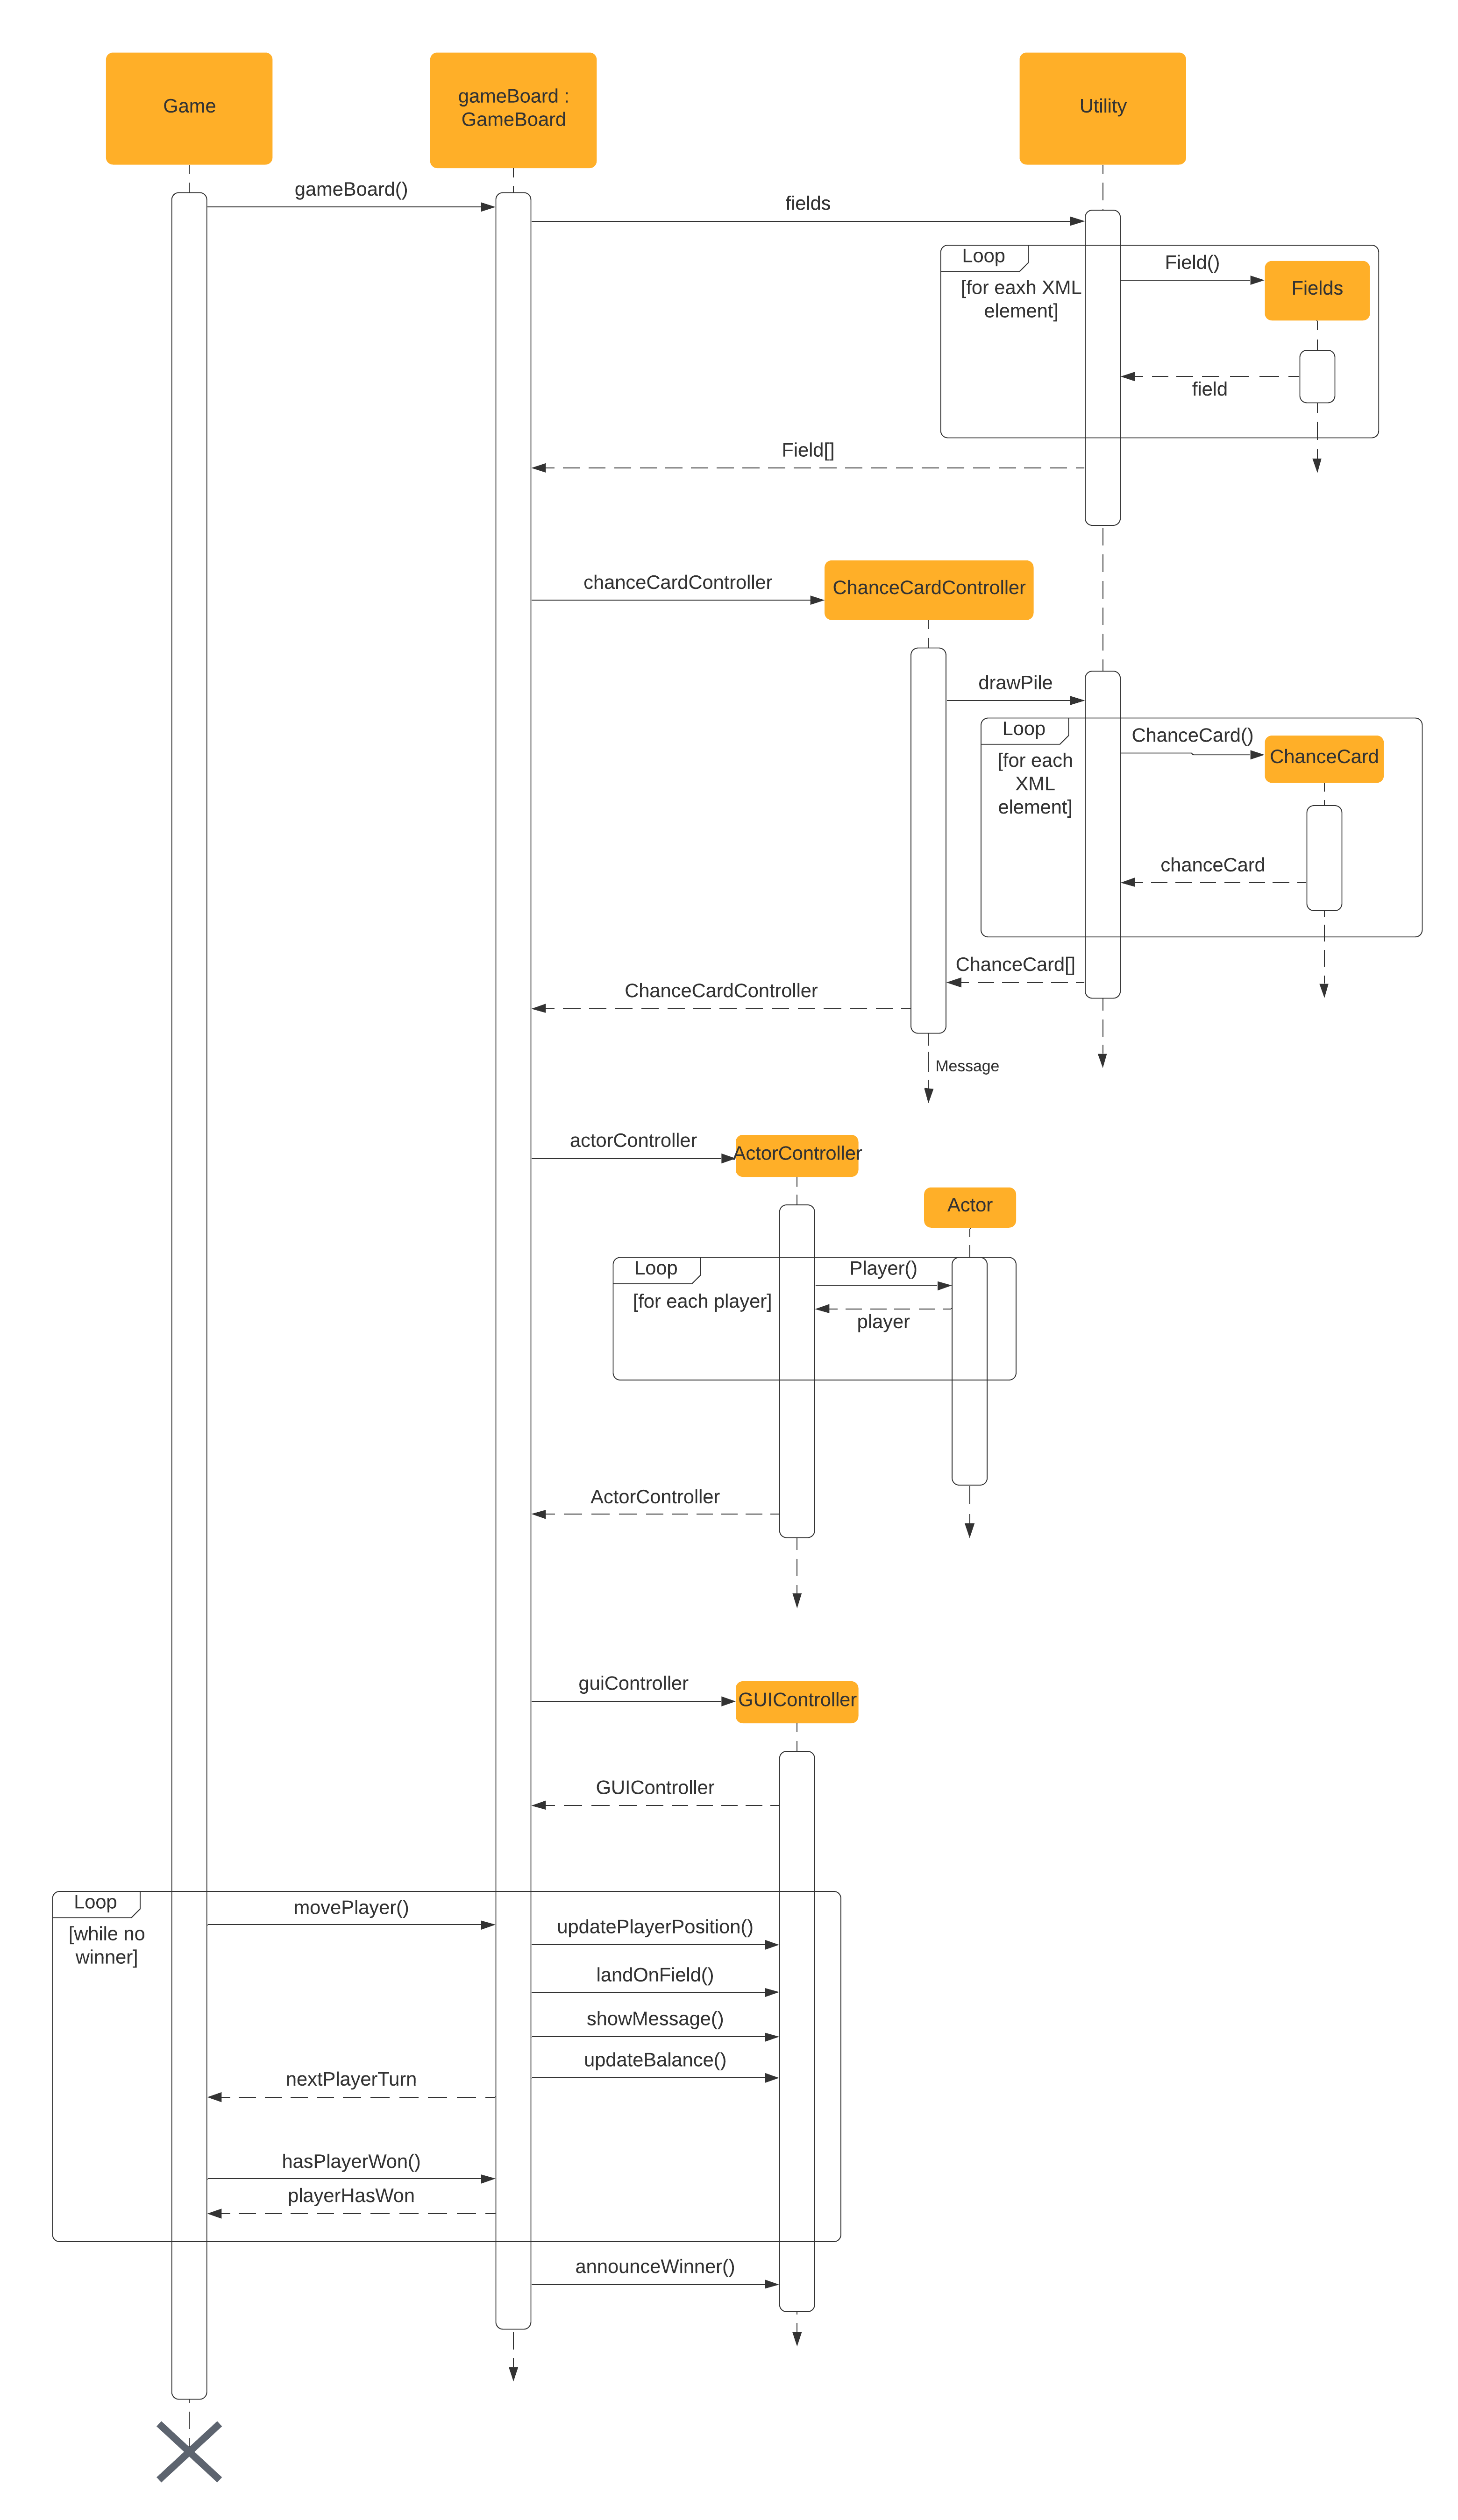
\includegraphics[scale=0.095]{artifacts/SD.png}
\end{figure}
\newpage
\section{Implementering} \label{implementation}
\subsection{Actors}
Da spillet nu skal udvides til et matadorspil har vi brug for en bank. Til dette er det oplagt at bruge nedarvning, da \texttt{Bank} og \texttt{Player} har mange metoder til fælles. Vi har derfor lavet en \texttt{Actor} som superklasse til de fælles attributter og metoder. Den er selvfølgelig \texttt{abstract} da vi ikke vil have lavet nogle instanser af den. \texttt{Bank} og \texttt{Player} klasserne nedarver således fra \texttt{Actor} klassen, så de begge kan få en start balance samt lave transactions.


\subsection{ActorController}
I metoden \texttt{makeTransaction} sikrer vi low coupling og high cohesion ved kun at tilgå de forskellige actors, transaktionen skal ske mellem gennem \texttt{ActorController}, mens det eneste \texttt{Actor} klassen gør når den bliver kaldt af \texttt{makeTransaction} er at udregne og sætte den nye balance for den instans af \texttt{Actor} som kalder metoden.

\subsection{GUIController}
Når man opretter et object af GUIController, skal der sendes en list af Fields med og antal af Fields, da det er GUIController, som skal starte GUI’en, og oprette de forskellige felter til spillet.
Inde i selve contructoren af klassen, vil der så være en switch case, som sørger for at tildele de forskellige felter den rigtige type af Field i GUI’en.
Derefter kan man kommunikere med GUI’en via det GUIController object man har lavet.
GUIControlleren opretter også spillere på den måde, at den spørger spillere om deres navn, og om man vil oprette flere spiller, derudover tjekker den også på, om man er noget max. Antal spiller, eller om man er under min. Antal spillere. Alle spillernavne bliver derefter smidt ind i et Array, som man kan hente med metode ”returnPlayerNames()”. 



\subsection{ChanceCardController}
Når man opretter et object a \texttt{ChanceCardController}, kommer dette til at indeholde et dæk med 20 chancekort. Man har mulighed for at trække et kort(som bliver returneret, da \texttt{GameBoard} skal håndtere hvad kortet gør), ved hjælp af \texttt{drawChanceCard()} metoden. Dækket bliver kørt igennem fra start til slut, og hvis der bliver kaldt \texttt{newGame()} bliver dækket blandet, og variable \texttt{cardsDrawn} bliver sat til 0, for at sørge for at man starter forfra med bunken.

\subsection{GameBoard}
Når \texttt{GameBoard} instantieres skal den bruge en liste af fields, hvilket den får fra \texttt{Utility} pakken, som læser felterne fra en xml fil. I konstruktøren bliver \texttt{GUIController} også instantieret, så et nyt vindue bliver lavet. 

Den centrale metode i \texttt{GameBoard} kan siges at være \texttt{fieldAction}, da det er den metode der eksekveres når spilleren lander på et spil og skal udføre en bestemt handling ud fra feltets type. Der er derfor forskellige metoder for de forskellige felter, som bliver kørt af \texttt{fieldAction}. 

Hver gang \texttt{fieldAction} bliver kaldt tjekkes der om nogen af spillerne er gået fallit ved at se om nogen af transaktionerne ikke er gået igennem. 

Hvis spilleren lander på et \texttt{Chance}felt skal der trækkes et chancekort som siger hvad spilleren skal gøre. I nogle tilfælde skal spilleren flytte sig frem på næste træk. Derfor bliver det gemt, og skal tjekkes for hver tur spillerne har.


I løbet af dette bliver \texttt{GUIController} også brugt til at ændre brættet i overensstemmelse med hvad der sker i spillets logik.
\subsection{Utility}
\texttt{Utility} indeholder methods til at hente data fra XML filer. Vi bruger Utility til at importere data til \texttt{ChanceCard} og \texttt{Field} objekterne, som skal bruges i programmet, samt til at lave \texttt{StringRef} objekter der skal benyttes af \texttt{StringHandler}. 

\subsection{StringHandler}
Denne object controller er lavet for at kunne søge på en String reference for at kunne hente den søgte String til brug hvor det er relevant (typisk i GUIController, der sender beskeder til udskrift i GUIen). Formålet med dette er at kunne skifte sproget fra engelsk til eksempelvis dansk ved blot at oversætte en række strenge i overskuelige filer (her XML).

\newpage
\section{Brug} \label{brug}
\begin{figure}
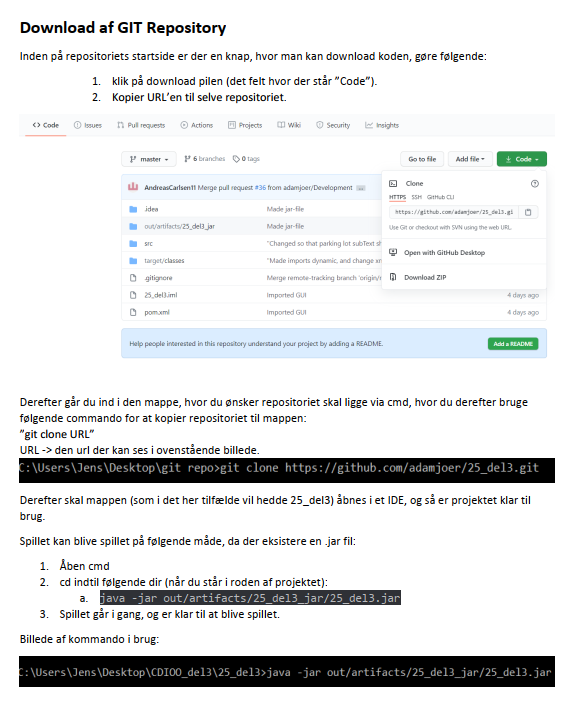
\includegraphics[scale=1]{artifacts/guide.png}
\end{figure}
\newpage
\section{Test} \label{test}
\subsection{Test cases}
\begin{figure}[h!]
\centering
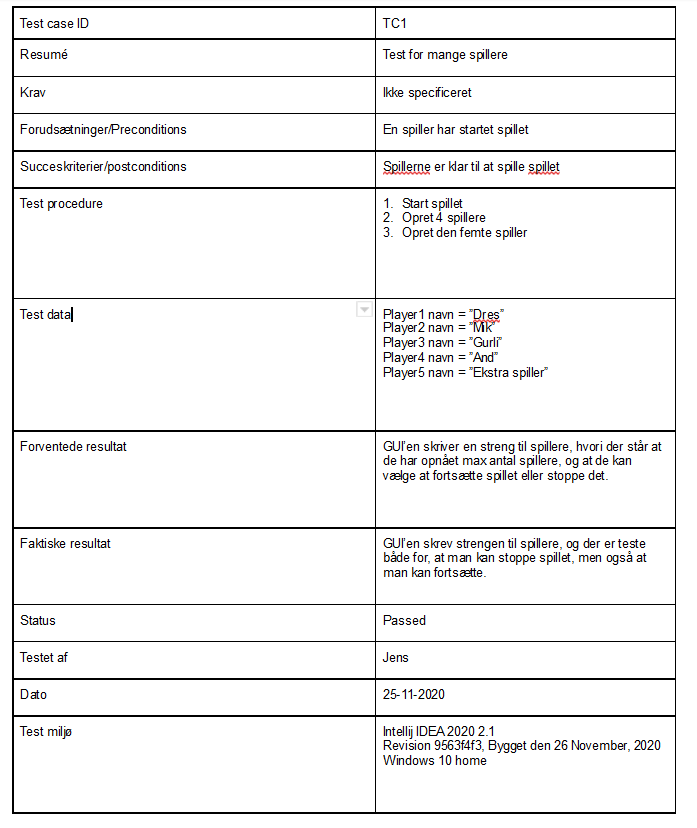
\includegraphics[scale=1]{artifacts/TC1.png}
\end{figure}

\newpage
\begin{figure}[h!]
\centering
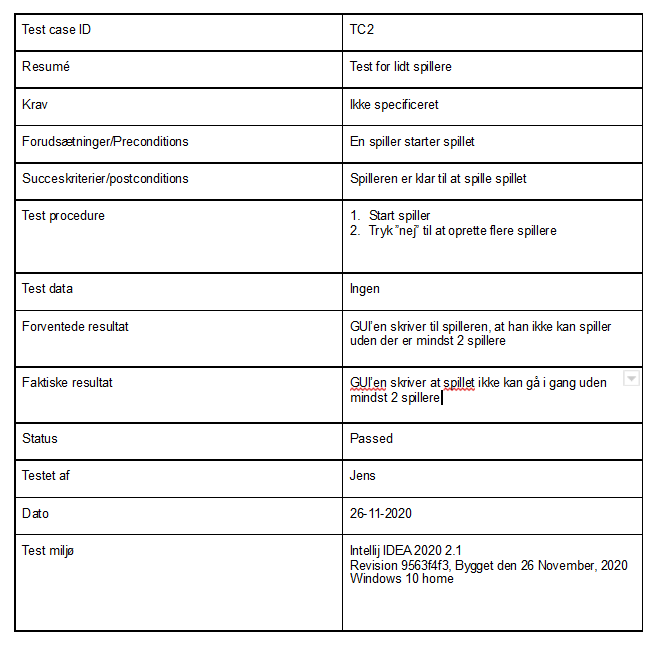
\includegraphics[scale=1]{artifacts/TC2.png}
\end{figure}

\newpage
\begin{figure}[h!]
\centering
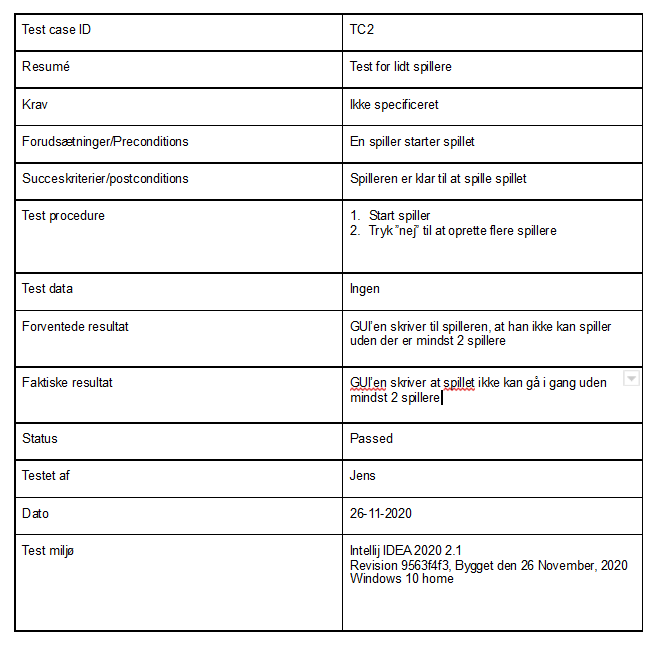
\includegraphics[scale=1]{artifacts/TC2.png}
\end{figure}
\newpage
\subsection{Dokumentation for code coverage}
\begin{figure}[h!]
\centering
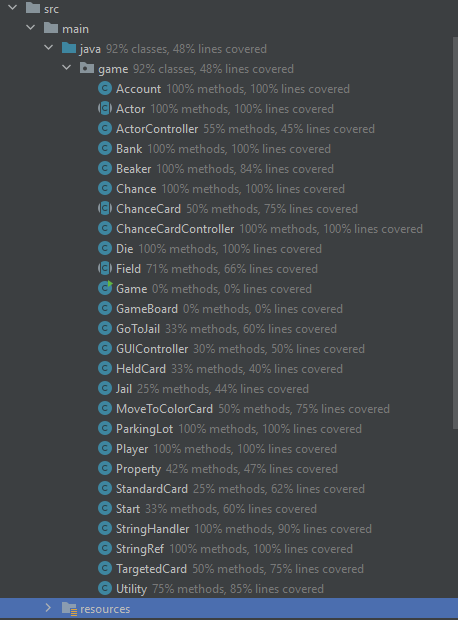
\includegraphics[scale=0.8]{artifacts/codeCoverageTest.png}
\end{figure}
\newpage
\section{Konklusion} \label{conclusion}
Vi har leveret et produkt, der forsøger at leve op til bestemte principper, herunder GRASP. Vi erfarer, at vores tilgang til udspecificering af krav har spændt ben for vores udviklingsarbejde, og denne erfaring tager vi med, således at vi fremover kan arbejde bedre efter et iterativt princip og med fokus på essentielle funktionaliteter først. Must have, should have, would have, could have - i den rækkefølge.

Vi har til trods for dette leveret et produkt, der stadig lever op til mange af de krav, der er blevet stillet - selvom vi har mangler.
\label{EndOfText}

\newpage
\pagenumbering{Roman} 
%\addcontentsline{toc}{section}{Figurer}
%\fancyfoot[C]{Page \thepage\ of \pageref{endOfDoc}}
%\listoffigures
%\thispagestyle{fancy}

%\newpage
%\addcontentsline{toc}{section}{Tabeller}
%\listoftables
%\thispagestyle{fancy}

%\newpage
%\addcontentsline{toc}{section}{Nomenklatur}
%\makenomenclature
\clearpage
\mbox{}

\nomenclature{EV}{Electric Vehicle}
\nomenclature{AC}{Alternating Current}
\nomenclature{DC}{Direct Current}
\nomenclature{IGBT}{Insulated-gate Bipolar Transistor}
\nomenclature{PV}{Photovoltaics}
\nomenclature{RMS}{Root Mean Square}
\nomenclature{FCS}{Fast Charging Station}
\nomenclature{PMU}{Phase Measurement Unit}
\nomenclature{THD}{Total Harmonic Distortion}
\nomenclature{EMI}{Electromagnetic Interference}
\nomenclature{$h$}{Planck constant}
 
\printnomenclature

%\newpage
\addcontentsline{toc}{section}{Litteratur}
%\printbibliography
\section*{Litteratur} \label{bibliography}
CDIO del 1

CDIO del 2
%\newpage
%\section{Bilag A} \label{ch11}

\label{endOfDoc}
\end{document}
